\documentclass[border=4pt]{standalone}
% Shared typography and colours for the standalone figures.
\usepackage{unicode-math}
\setmainfont{TeX Gyre Termes}
\setmathfont{TeX Gyre Termes Math}
\usepackage{tikz}
\usetikzlibrary{arrows.meta,positioning,calc,decorations.pathreplacing}
\usepackage{pgfplots}
\pgfplotsset{compat=1.18}
\definecolor{elemA}{HTML}{1F5FA8}
\definecolor{elemB}{HTML}{B8461B}
\definecolor{elemC}{HTML}{2E7D32}
\definecolor{elemD}{HTML}{6A4C93}
\definecolor{frameline}{HTML}{555555}

\begin{document}
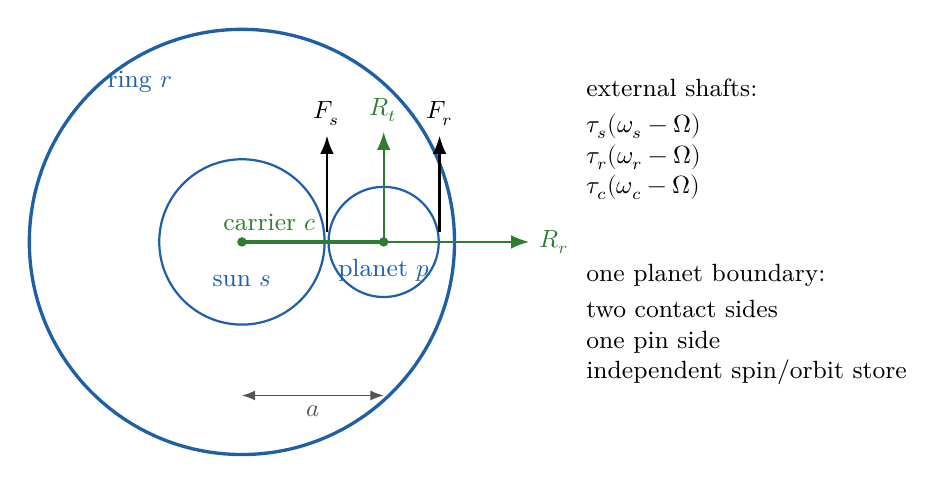
\begin{tikzpicture}[>=Latex,font=\small]
\draw[very thick,elemA] (0,0) circle (2.7);
\draw[thick,elemA] (0,0) circle (1.05);
\draw[thick,elemA] (1.8,0) circle (.7);
\draw[very thick,elemC] (0,0)--(1.8,0);
\fill[elemC] (0,0) circle (.06);
\fill[elemC] (1.8,0) circle (.06);
\node[elemA] at (0,-.5) {sun $s$};
\node[elemA] at (1.8,-.36) {planet $p$};
\node[elemA] at (-1.3,2.03) {ring $r$};
\node[elemC,above] at (.35,.02) {carrier $c$};
\draw[->,thick] (1.08,.12)--(1.08,1.35) node[above] {$F_s$};
\draw[->,thick] (2.51,.12)--(2.51,1.35) node[above] {$F_r$};
\draw[->,thick,elemC] (1.8,0)--(1.8,1.4) node[above] {$R_t$};
\draw[->,thick,elemC] (1.8,0)--(3.65,0) node[right] {$R_r$};
\draw[<->,frameline] (0,-1.95)--(1.8,-1.95) node[midway,below] {$a$};
\node[align=left,anchor=west] at (4.25,1.3)
 {external shafts:\\[2pt]$\tau_s(\omega_s-\Omega)$\\$\tau_r(\omega_r-\Omega)$\\$\tau_c(\omega_c-\Omega)$};
\node[align=left,anchor=west] at (4.25,-1.05)
 {one planet boundary:\\[2pt]two contact sides\\one pin side\\independent spin/orbit store};
\end{tikzpicture}
\end{document}
